\section*{Постановка задачи}
Реализовать консольное приложение с алгоритмами сортировки на динамически
типизированном языке, повторить и изучить основные конструкции языка.

Установить Python и среду разработки.

Реализовать алгоритм сортировки выбором и вставкой.
\addcontentsline{toc}{section}{Постановка задачи}

\section{Алгоритм решения}
Для того, чтобы что-то сортировать нам необходимы входные данные.
Воспользуемся стандартными функциями Python для генерации случайных чисел.
Сохраним эти числа в файл, чтобы потом отсортировать его.
Сортировку будет производить с данными из файла со случайными числами.
Комплекс программ будет работать вот так:

\begin{verbatim}
    $ ./random_numbers.py min max count > output.txt
    $ time ./selection_sort.py < output.txt
    $ time ./insert_sort.py < output.txt
\end{verbatim}

Сначала запустим программу \verb|random_number.py| с параметрами \verb|min|, \verb|max| и \verb|count|.
Параметры нужно заменить на аргументы (целые числа).
Вывод программы запишем в файл \verb|output.txt|.
Затем запустим программу \verb|time| для того, чтобы засечь время выполнения сортировки.
Программа сортировки принимает на вход поток из строк, которые мы будем сортировать.

Вот конкретный пример запуска:

\begin{verbatim}
    $ ./random_numbers.py 0 10 5 > tmp
    $ cat tmp
    5
    1
    2
    3
    4
    $ time ./selection_sort.py < tmp
    1
    2
    3
    4
    5
    
    real    0m0.034s
    user    0m0.026s
    sys     0m0.008s
    $ time ./insertion_sort.py < tmp
    1
    2
    3
    4
    5
    
    real    0m0.062s
    user    0m0.051s
    sys     0m0.005s
    $ time sort < tmp
    1
    2
    3
    4
    5
    
    real    0m0.010s
    user    0m0.005s
    sys     0m0.004s
\end{verbatim}

Программа \verb|time| возвращает данные в трёх значениях.
Эти статистические данные состоят из времени, прошедшего в реальном времени
между вызовом и его завершением, процессорного времени пользователя и системного
процессорного времени.

В последнем примере была использована стандартная утилита GNU для сортировки.
Она реализует многопоточный алгоритм сортировки.
Как видим, на машине с 8 потоками, она работает быстрее наших алгоритмов
сортировки.

\subsection{Сортировка выбором}

В информатике сортировка по выбору --- это алгоритм сортировки сравнения на месте.
Она имеет временную сложность $O(n^2)$, что делает ее неэффективной в больших
списках и, как правило, работает хуже, чем аналогичная сортировка вставкой.
Сортировка по выбору отличается своей простотой и имеет преимущества в
производительности по сравнению с более сложными алгоритмами в определенных
ситуациях, особенно когда вспомогательная память ограничена.

Алгоритм делит входной список на две части: отсортированный подсписок элементов,
который создается слева направо в начале (слева) списка, и подсписок оставшихся
несортированных элементов, которые занимают остальную часть списка.
Первоначально отсортированный подсписок пуст, а несортированный подсписок
представляет собой весь входной список. Алгоритм заключается в нахождении
наименьшего (или наибольшего, в зависимости от порядка сортировки) элемента в
несортированном подсписке, замене его крайним левым несортированным
элементом (размещении его в отсортированном порядке) и перемещении границ
подсписка на один элемент вправо.

Временная эффективность сортировки по выбору квадратична, поэтому существует ряд
методов сортировки, которые имеют лучшую временную сложность, чем сортировка по
выбору. Одна вещь, которая отличает сортировку по выбору от других алгоритмов
сортировки, заключается в том, что она выполняет минимально возможное количество
обменов, $n-1$ в худшем случае.

Вот пример такого алгоритма сортировки, сортирующего пять элементов:

\begin{table}[H]
    \begin{tabular}{|l|r|l|}
        \hline
        \begin{tabular}[c]{@{}l@{}}Сортированный\\ подсписок\end{tabular}                        &
        \multicolumn{1}{l|}{\begin{tabular}[c]{@{}l@{}}Несортированный\\ подсписок\end{tabular}} &
        \begin{tabular}[c]{@{}l@{}}Наименьший элемент \\ в несортированном списке\end{tabular}                               \\ \hline
        ()                                                                                       & (11, 25, 12, 22, 64) & 11 \\ \hline
        (11)                                                                                     & (25, 12, 22, 64)     & 12 \\ \hline
        (11, 12)                                                                                 & (25, 22, 64)         & 22 \\ \hline
        (11, 12, 22)                                                                             & (25, 64)             & 25 \\ \hline
        (11, 12, 22, 25)                                                                         & (64)                 & 64 \\ \hline
        (11, 12, 22, 25, 64)                                                                     & ()                   &    \\ \hline
    \end{tabular}
\end{table}

Сортировка выбором также может использоваться со списками, которые повышают
эффективность добавления и удаления. В этом случае чаще всего минимальный
элемент удаляется из оставшейся части списка, а затем вставляется в конец
отсортированных значений. Например:

\begin{verbatim}
    arr[] = 64 25 12 22 11

    // Найдите минимальный элемент в arr[0...4]
    // и поместите его в начало
    11 25 12 22 64

    // Найдите минимальный элемент в arr[1...4]
    // и поместите его в начало arr[1 ...4]
    11 12 25 22 64

    // Найдите минимальный элемент в arr[2...4]
    // и поместите его в начало arr[2 ...4]
    11 12 22 25 64

    // Найдите минимальный элемент в arr[3...4]
    // и поместите его в начало arr[3 ...4]
    11 12 22 25 64 
\end{verbatim}

Сортировка по выбору не сложна для анализа по сравнению с другими алгоритмами
сортировки, поскольку ни один из циклов не зависит от данных в массиве. Для
выбора минимального элемента требуется сканирование $n$ элементов ($n-1$
сравнение), а затем замена его на первую позицию. Для поиска следующего
наименьшего элемента требуется сканирование оставшихся $n-1$ элементов и так
далее. Таким образом, общее количество сравнений равно

$$(n-1)+(n-2)+...+1=\sum _{i=1}^{n-1}i$$

По арифметической прогрессии,

$$\sum
    _{i=1}^{n-1}i={\frac{(n-1)+1}{2}}(n-1)={\frac{1}{2}}n(n-1)={\frac{1}{2}}(n^{2}-n)$$

имеет сложность $O(n^{2})$ с точки зрения количества сравнений. Для
каждого из этих сканирований требуется одна замена $n-1$ элементов (последний
элемент уже не надо сравнивать).

\subsection{Сортировка вставкой}

Сортировка вставкой --- это простой алгоритм сортировки, который создает
отсортированный массив (или список) по одному элементу за раз. Он гораздо менее
эффективен для больших списков, чем более продвинутые алгоритмы, такие как
быстрая сортировка, пирамидальная сортировка или сортировка слиянием. Однако
сортировка по вставке дает несколько преимуществ:

\begin{itemize}
    \item Эффективен для небольших наборов данных, так же, как и другие квадратичные алгоритмы сортировки
    \item Более эффективен на практике, чем большинство других простых квадратичных алгоритмов, таких как сортировка по выбору или сортировка пузырьком
    \item Адаптивный, т.е. эффективен для почти отсортированных данных: временная сложность составляет $O(kn)$, где $k$ - количество мест неотсортированных позиций
    \item Стабильный, т.е. не изменяет относительный порядок одинаковых элементов
    \item Не требует дополнительной памяти, т.е. может сортировать на месте (как и алгоритм сортировки выбором)
    \item Автономен, т.е. может сортировать список по мере его получения
\end{itemize}

\section{Тестирование программы}

\begin{figure}[H]
    \begin{center}
        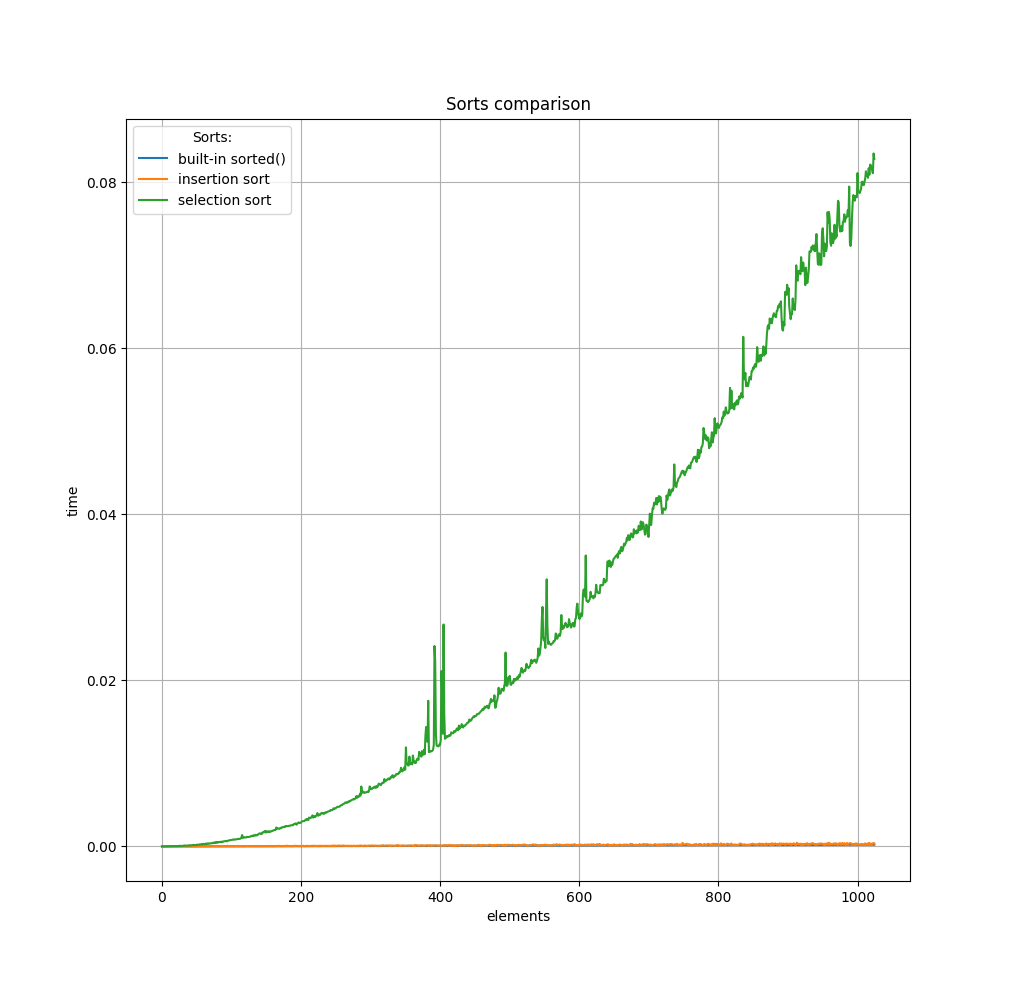
\includegraphics[scale=0.5]{Figure_1}
        \caption{Результат сортировки. На графике 3 функции: встроенная в Python
            сортировка, сортировка вставками и сортировка выбором}
    \end{center}
\end{figure}

\begin{figure}[H]
    \begin{center}
        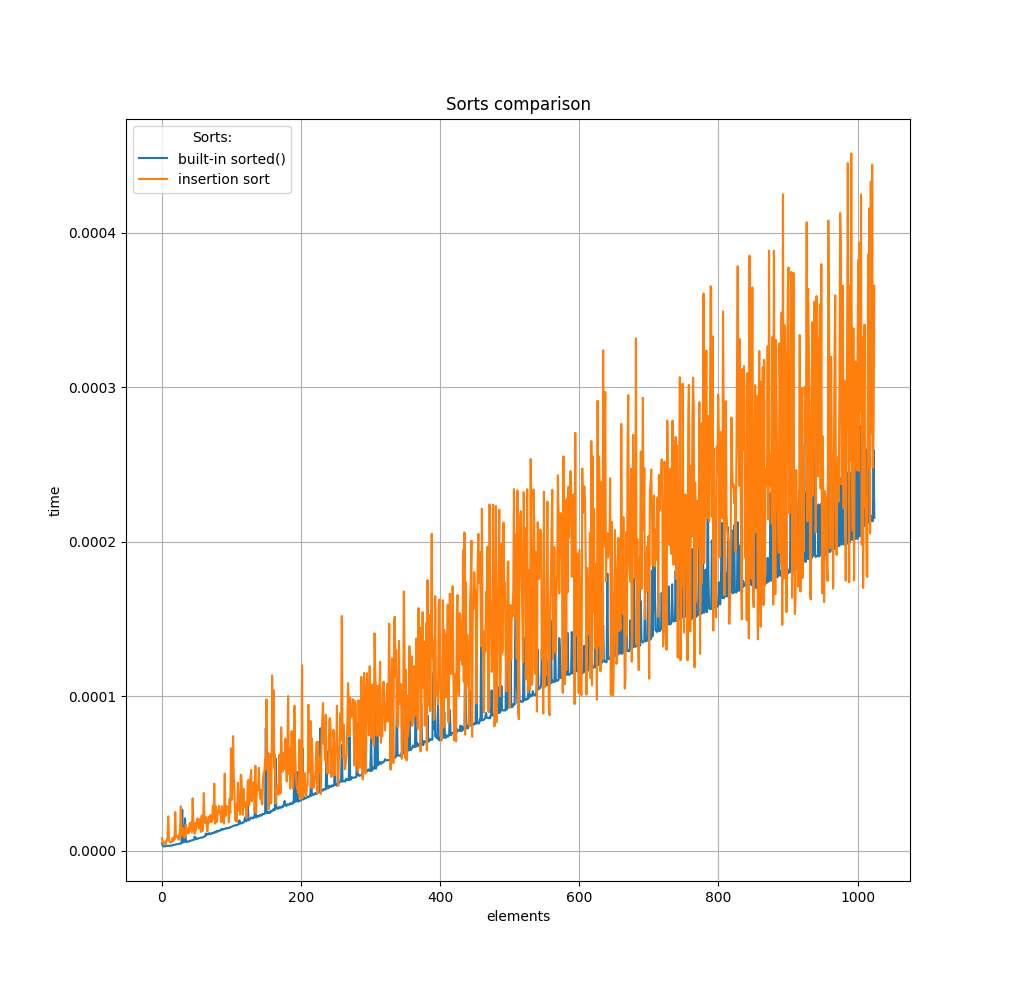
\includegraphics[scale=0.5]{Figure_2}
        \caption{Результат сортировки. На графике 2 функции: встроенная в Python
            сортировка и сортировка вставками}
    \end{center}
\end{figure}

По графикам видно, что встроенная сортировка \verb|Python| более стабильна.
Нет такого большого разброса по времени.

Теперь демонстрация записи в файл:

\begin{verbatim}
    # генерация файла со случайным набором чисел
    $ ./random_number.py -10 10 5 > data
    # ввод файла с данными в программу сортировки чисел и вывод отсортированных
    # данных
    $ cat data | ./selection_sort.py > selection_data
    $ cat data | ./insertion_sort.py > insertion_data
    # расчёт времени работы сортировки
    $ time ( ./insertion_sort.py < data > insertion_data )
    ( ./insertion_sort.py < data > insertion_data; ) 0.05s user 0.01s system
    173% cpu 0.037 total
\end{verbatim}

Ссылка на репозиторий с программами и отчёт написанный с помощью \LaTeX:
\url{https://github.com/andreymlv/tstu-computation-theory}

\section*{Заключение}
Реализовали две квадратичные сортировки. Из графиков видно, что встроенная
функция сортировки \verb|Python| работает в разы стабильнее и эффективнее по
времени.

Установили \verb|Python 3.10.6|, среду разработки \verb|VSCode|, библиотеку
\verb|Dear PyGui| для графического интерфейса, а так же использовали сторонний
пакетный менеджер \verb|Poetry| для изоляции от глобально установленных пакетов.
\addcontentsline{toc}{section}{Заключение}